\section{Introduction}
\subsection{Cette présentation}
\begin{frame}
  \frametitle{Parties falculatives}
  \begin{center}
      \Warning = Information facultative (non couverte par l'orateur)
  \end{center}
\end{frame}
\subsection{Qu'est-ce que \LaTeX{}?}

\begin{frame}
\frametitle{Qu'est-ce que \LaTeX}
\begin{itemize}
\item \LaTeX{} $=$ méthode privilégiée d'écriture de documents scientifiques
 \vspace{0.5cm}
\item \LaTeX{} $ \neq$ WYSIWYG (What You See Is What You Get)
\end{itemize}
\end{frame}

%-----------------------
\subsection{Pourquoi \LaTeX{}?}

\begin{frame}{Pourquoi \LaTeX{}?}
  \begin{itemize}
      \item Documents de qualité professionnelle
    \item Facilité d'emploi des :
    \begin{itemize}
        \item formules mathématiques
        \item tables des matières
        \item images et tableaux
        \item références bibliographiques
        \item références croisées
        \item \ldots{}
    \end{itemize}
    \item Gratuit
    \item Stable, même pour les très gros documents
  \end{itemize}
\end{frame}


\begin{frame}{Pourquoi \LaTeX{}?}
\begin{figure}[htbp]
\begin{center}
\includegraphics[height=6.5cm]{img/latex_exemples.jpg}
\end{center}
\end{figure}
\end{frame}

%-----------------------
\subsection{Pourquoi pas \LaTeX{}?}

\begin{frame}{Pourquoi pas \LaTeX{}?}
  \begin{itemize}
    \item Prise en main plus longue que pour traitement de texte WYSIWYG
    \item Je suis allergique à toute forme de code informatique
    \item J'ai des actions Microsoft
    \item Je ne trouve pas le ``\textbackslash'' sur mon clavier
  \end{itemize}
\end{frame}

\begin{comment}
\begin{frame}{Oui mais\ldots{}}
  \begin{center}
    %\resizebox{\textwidth}{!}{
    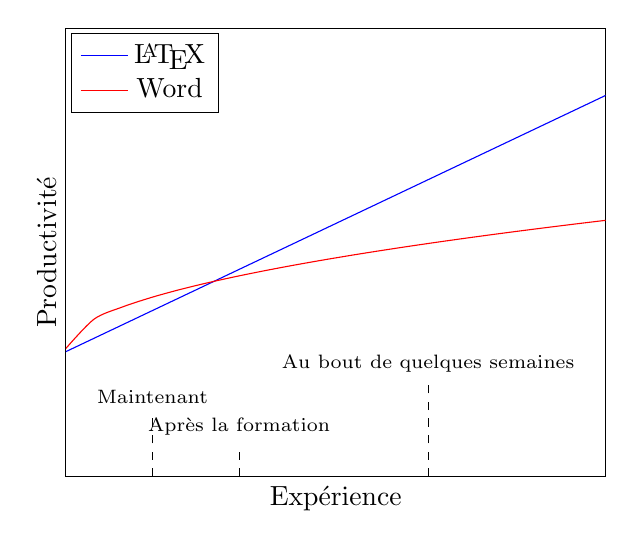
\begin{tikzpicture}
      \begin{axis}[xmin=0, xmax=4, ymin=-2, ymax=5, ticks=none,
          xlabel={Expérience}, ylabel=Productivité,
        legend style={at={(0.01,0.99)}, anchor=north west}]
        \addplot[smooth, color=blue]{x-0.05};
        \addlegendentry{\LaTeX}
        \addplot[smooth, color=red,domain=0:5]{sqrt(x)};
        \addlegendentry{Word}
        %\xlabel{Productivité}
        %\ylabel{Expérience/maitrise}
      \end{axis}
      \foreach \x/\com/\deltax/\deltay/\adj in {
        %\small
        {1.1}/{\scriptsize Maintenant}/{0}/{0.8}/below,
        {2.2}/{\scriptsize Après la formation}/{0}/{0.4}/below,
        %{4.6}/{À l'heure de votre mémoire}/{0}/{1.2}/below
        {4.6}/{\scriptsize Au bout de quelques semaines}/{0}/{1.2}/below
      } {
        %\fill \coord circle (100pt) node[\adj] {$\coord$};
        \draw[dashed] (\x,0) -- (\x+\deltax,\deltay) node[above] {\com};
        %\draw (\x+\deltax,\deltay) node {\com};
      }
    \end{tikzpicture}
    %}
  \end{center}
\end{frame}
\end{comment}

%-----------------------
\subsection{Les Outils}

\begin{frame}{\Warning Quels logiciels pour utiliser \LaTeX{}?}
  \begin{itemize}
      \item GNU/Linux
      \begin{itemize}
          \item Distribution \LaTeX{} : \textbf{TeXLive}
          {\tiny (\lstinline|sudo apt install texlive-full|)}
        \item Éditeur : \textbf{\href{http://www.xm1math.net/texmaker/}{TeXMaker}}
      \end{itemize}
      \item Windows
      \begin{itemize}
        \item Distribution \LaTeX{} : \textbf{TeXLive}
        \item Éditeur : \textbf{\href{http://www.xm1math.net/texmaker/}{TeXMaker}}
      \end{itemize}
      \item Mac OS
      \begin{itemize}
        \item Distribution \LaTeX{} : \textbf{\href{https://www.tug.org/mactex/}{MacTeX}}
        \item Éditeur : \textbf{\href{http://www.xm1math.net/texmaker/}{TeXMaker}}
      \end{itemize}
    \end{itemize}
\end{frame}

\begin{frame}{Overleaf}
  Pour cet atelier, nous vous conseillons d'utiliser \textbf{overleaf} sur votre propre PC.
  \begin{center}
    \textbf{\url{www.overleaf.com}}
  \end{center}
  Vous pouvez déjà vous créer un compte (gratuit!)
\end{frame}
%-----------------------
\subsection{Symboles spéciaux sur Mac}

\begin{frame}{Symboles spéciaux sur Mac}
  \begin{center}
    \begin{tabular}{|lc|l|}
      \hline
      Symbole & & Raccourci clavier \\\hline
      \textit{backslash} & \textbackslash & option + shift + / \\
      accolade & \{\} & option + () \\
      crochet & $[]$ & option + shift + () \\
      \textit{pipe} & | & option + shift + L \\
      \hline
    \end{tabular}
  \end{center}
\end{frame}
